\documentclass{article}

\usepackage{color}
\usepackage{amsmath}
\usepackage{graphicx}
\usepackage{float}
\usepackage{wrapfig}
\usepackage{csquotes}
\usepackage{amssymb}




\title {CSE300\textunderscore Assignment1\\Introduction to\LaTeX\\Albert Einstein}
\author{Subangkar Karmaker Shanto\\Student ID: 1505015}

\date{}

\begin{document}
\begin{titlepage}
\maketitle
\thispagestyle{empty}
\null
\vfill
\begin{figure}[h]
    \centering
    
\includegraphics[width=.25\textwidth]{figures/logoBIRN.png}
    \label{fig:logo}
\end{figure}
\begin{center}
Department of Computer Science and Engineering \\Bangladesh University of Engineering and Technology\\(BUET)\\Dhaka 1000 \\
\date{\today}
    
\end{center}
\end{titlepage}

\newpage

\tableofcontents

\newpage


\section{\textcolor{magenta}{Introduction}}

\begin{displayquote}
"Everybody is a genius. But if you judge a fish by its ability to climb a tree, it will live its whole life believing that it is stupid." - {\textit{Albert Einstein}}
\end{displayquote}





\begin{wrapfigure}{r}{0.55\textwidth}
\vspace{-10pt}

\begin{center}
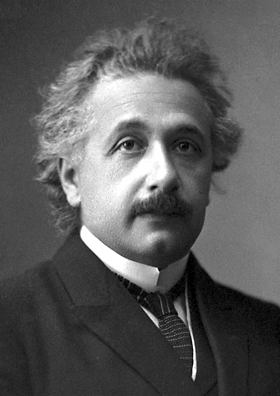
\includegraphics[width=.5\textwidth]{figures/Albert_Einstein__Nobel_.png}
\end{center}

\vspace{-10pt}
\caption{Albert Einstein}
\vspace{-10pt}
\end{wrapfigure}

\textbf{Albert Einstein} (14 March 1879 {-} 18 April 1955) was a German-born theoretical physicist who developed the theory of relativity, one of the two pillars of modern physics (alongside quantum mechanics). His work is also known for its influence on the philosophy of science.He is best known by the general public for his mass energy equivalence formula \textbf{$ E = mc^2 $} (which has been dubbed \textbf{\textit{"the world's most famous equation"}}).He received the \textcolor{red}{\textbf{1921 Nobel Prize in Physics}} \textit{"for his services to theoretical physics, and especially for his discovery of the law of the photoelectric effect"}, a pivotal step in the evolution of quantum theory.


Einstein published more than \textcolor{blue}{300 scientific papers} along with over 150 non-scientific works. His intellectual achievements and originality have made the word "Einstein" synonymous with "genius". Eugene Wigner wrote of Einstein in comparison to his contemporaries that "Einstein's understanding was deeper even than Jansci von Neumann's. His mind was both more penetrating and more original than von Neumann's. And that is a very remarkable statement."



\section{\textcolor{magenta}{Life and career}}

\subsection{Timeline}
\begin{description}

\item[Mystery of Magnetism(1884)]
At the age of five, Albert Einstein becomes fascinated by his father's pocket compass, intrigued by invisible forces that cause the needle always to point north. Later in life, Einstein will look back at this moment as the genesis of his interest in science.

\item[Move to Italy(1894)]
Struggling financially, the Einstein family moves from Germany to Italy in search of better work. Albert, aged fifteen, stays behind in Munich to finish his schooling, but soon either quits or is kicked out of his high school and follows his parents to Italy.

\item[Boarding School in Aarau(1895)]
Albert Einstein attempts to get out of his last year of high school by taking an entrance exam to ETH, the Swiss Polytechnic University in Zurich. He fails the test, forcing him to attend one final year of high school in the small town of Aarau, Switzerland, instead.

\item[Einstein at ETH(1896)]
Albert Einstein graduates from high school and begins attending ETH, the prestigious Swiss Polytechnic University in Zurich.

\item[Einstein Renounces German Citizenship(1896)]
At the age of 17, Albert Einstein renounces his German citizenship to avoid mandatory military service in the German army. For the next four years, he will not be a legal citizen of any nation.

\item[College Graduation(1900)]
Albert Einstein graduates from ETH with a degree in physics. He tries to find a teaching job, but is unable to obtain work.

\item[Einstein Impregnates Girlfriend(1901)]
Albert Einstein travels to Italy for a tryst with his on-again, off-again girlfriend, Milena Maric, a former classmate at the ETH. He ends up getting her pregnant.

\item[Daughter Born, Put Up for Adoption(1902)]
Milena Maric gives birth to Leiserl Einstein, Albert's first child. The unwed couple, unable to care for the girl and perhaps ashamed of her illegitimate status, put her up for adoption.

\item[Swiss Patent Office(1902)]
Unable to find any work as a teacher or academic, Albert Einstein takes a job as a clerk at the Swiss Patent Office.

\item[Einstein Marries Milena Maric(1903)]
Albert Einstein marries his longtime girlfriend, Milena Maric.

\item[Birth of Hans Albert Einstein(1904)]
A year after marrying Albert, his wife Milena gives birth to the Einsteins' first son, Hans Albert.

\item[Annus Mirabilis(1905)]
Over the course of a year that he will later describe as his "Annus Mirabilis"—his miraculous year—Albert Einstein publishes four major theoretical papers in the prestigious German academic journal Annalen Der Physik. The four papers include a groundbreaking new interpretation of the photoelectric effect (for which Einstein will eventually win the Nobel Prize) as well as the first published exploration of the theory of Special Relativity and the first formulation of the famous equation
$ E = mc^2 $


\item[Birth of Eduard Einstein(1910)]
Albert Einstein's wife Milena gives birth to their second son, Eduard.

\item[General Theory of Relativity(1915)]
Einstein completes his General Theory of Relativity.

\item[Divorce and Remarriage(1919)]
After several years of estrangement, Albert divorces his first wife Milena Maric and immediately remarries. Einstein's second wife, Elsa Lowenthal, is a cousin with whom he fell in love when she nursed him back to health following a serious illness in 1917.

\item[Restoration of German Citizenship(1919)]
At the close of World War I, Albert Einstein regains his German citizenship in a gesture of solidarity with liberal new government of the Weimar Republic.

\item[Eclipse Proves Theory of Relativity(\date{May 29, 1919})]
A solar eclipse provides dramatic observable evidence that Einstein's General Theory of Relativity is correct. Einstein suddenly becomes a worldwide celebrity.

\item[Nobel Prize(1921)]
Albert Einstein wins the Nobel Prize in Physics for his work on the photoelectric effect, first published in 1905.

\item[Escape from Nazi Germany(1933)]
Albert Einstein and his family, fearing anti-Semitic persecution, flee from Nazi Germany to resettle in the United States. Einstein takes a post at Institute of Advanced Study at Princeton, where he will remain until his death in 1955.

\item[Death of Elsa Einstein(1936)[]
Albert Einstein's second wife Elsa dies of sudden illness.

\item[Letter to President Roosevelt(1939)]
\begin{figure}[b!]
    \centering
    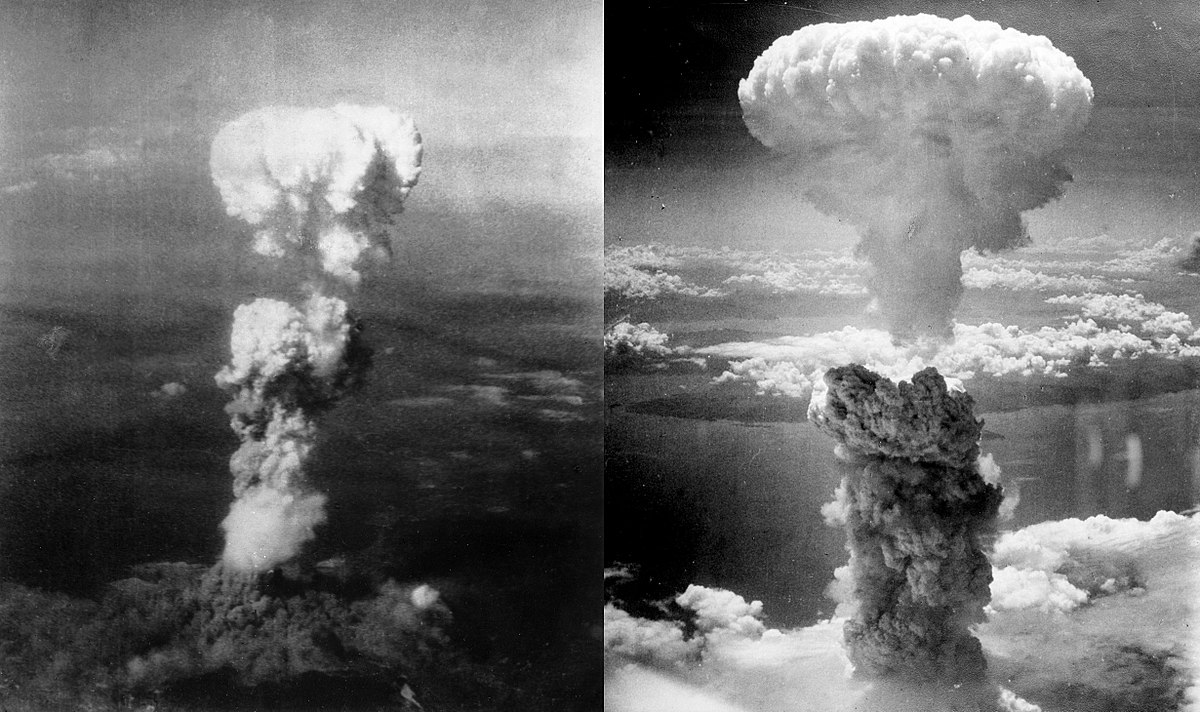
\includegraphics[width=10cm,height=6cm]{figures/1200px-Atomic_bombing_of_Japan.jpg}
    \caption{Atomic Bomb Explosion in Hiroshima(left) and Nagasaki(right) during World War II}
    \label{fig:atomic_explode}
\end{figure}
Fearing that Nazi scientists might win the race to develop the world's first atomic bombs, Albert Einstein writes a letter to President Franklin D. Roosevelt, urging him to launch an American program of nuclear research.
That eventually led to the use of atomic weapons in 1945 in Japan[Figure-\ref{fig:atomic_explode}] by the US Army.


\item[US Citizenship(1940)]
For the third time in his life, Albert Einstein changes his nationality, becoming a United States citizen while also retaining his Swiss citizenship.

\item[Death of Albert Einstein(\date{Apr 18, 1955})]
Albert Einstein dies of heart failure at the age of 76.
\end{description}


\subsection{Academic career}
\subsubsection{First scientific papers}
In 1900, Einstein's paper "Folgerungen aus den Capillaritätserscheinungen" ("Conclusions from the Capillarity Phenomena") was published in the journal Annalen der Physik.On 30 April 1905, Einstein completed his thesis, with Alfred Kleiner, Professor of Experimental Physics, serving as pro-forma advisor. As a result, Einstein was awarded a PhD by the University of Zürich, with his dissertation "A New Determination of Molecular Dimensions".

In that same year, which has been called Einstein's annus mirabilis (miracle year), he published four groundbreaking papers, on the photoelectric effect, Brownian motion, special relativity, and the equivalence of mass and energy, which were to bring him to the notice of the academic world, at the age of 26.

\begin{flushleft}
By 1908, he was recognized as a leading scientist and was appointed lecturer at the University of Bern. The following year, after giving a lecture on electrodynamics and the relativity principle at the University of Zürich, Alfred Kleiner recommended him to the faculty for a newly created professorship in theoretical physics. Einstein was appointed associate professor in 1909.

~\newline
Einstein became a full professor at the German Charles-Ferdinand University in Prague in April 1911, accepting Austrian citizenship in the Austro-Hungarian Empire to do so.During his Prague stay, he wrote 11 scientific works, five of them on radiation mathematics and on the quantum theory of solids. In July 1912, he returned to his alma mater in Zürich. From 1912 until 1914, he was professor of theoretical physics at the ETH Zurich, where he taught analytical mechanics and thermodynamics. He also studied continuum mechanics, the molecular theory of heat, and the problem of gravitation, on which he worked with mathematician and friend Marcel Grossmann.
\end{flushleft}




\section{\textcolor{magenta}{Scientific career}}

Throughout his life, Einstein published hundreds of books and articles. He published more than 300 scientific papers and 150 non-scientific ones.On 5 December 2014, universities and archives announced the release of Einstein's papers, comprising more than 30,000 unique documents. Einstein's intellectual achievements and originality have made the word "Einstein" synonymous with "genius". In addition to the work he did by himself he also collaborated with other scientists on additional projects including the Bose–Einstein statistics, the Einstein refrigerator and others.Einstein will never be forgotten for his remarkable contributions in the following fields \& innovations:

\newpage
\subsection{Major Innovations}
\begin{description}

\item[Theory of relativity]
\begin{equation}
    E = mc^2
\label{eqn:emc}
\end{equation}
Equation\eqref{eqn:emc} is the mass energy equivalence formula which brought him the Nobel prize in 1921.

\item [General relativity and the equivalence principle]
\begin{equation*}
    R \type_{\mu \nu} - R g \type_{\mu \nu} = \frac{8 \pi G}{c^4} T \type_{\mu \nu}
\end{equation*}

\item [Modern quantum theory]
\begin{equation}
     \int_{-\infty}^{\infty} \Psi (x,t)^ * \Psi (x,t) dx = 1 
    \label{eqn:wave_prob_dst}
\end{equation}
    Equation\eqref{eqn:wave_prob_dst} is the equation of wave function which is the basis of quantum mechanics.
\end{description}
\subsection{Others}
\begin{enumerate}
    \item Wave–particle duality
    \item Thermodynamic fluctuations and statistical physics
    \item Photons and energy quanta
    \item Quantized atomic vibrations
    \item Adiabatic principle and action-angle variables
    \item Theory of critical opalescence
    \item Zero-point energy
    \item Hole argument and Entwurf theory
    \item Physical cosmology
    \item Bose–Einstein statistics
    \item Energy momentum pseudotensor
    \item Unified field theory
    \item Wormholes
    \item Einstein–Cartan theory
    \item Equations of motion
    \item Einstein–Podolsky–Rosen paradox
\end{enumerate}



\section{\textcolor{magenta}{Awards and honors}}
Einstein received numerous awards and honors. Some popular of those are followings:

\begin{itemize}
    \item Nobel Prize in Physics, 1921. 
    \item Admission to German Order "Pour La Mérite," 1923. 
    \item Copley Medal, Royal Society of London, 1925. 
    \item Gold Medal, Royal Astronomical Society, London, 1925. 
    \item Max-Planck-Medal, German Physical Society, 1929. 
    \item Benjamin Franklin Medal, Franklin Institute, Philadelphia, 1935
\end{itemize}


\end{document} 